\documentclass[../../main.tex]{subfiles}
\graphicspath{{images/Maschinentechnik/}{../../images/Maschinentechnik/}}

\lstset{basicstyle=\small,
      showstringspaces=false,
      commentstyle=\color{black},
      keywordstyle=\color{blue}
    }

\begin{document}
    \subsection{Fahrwerk}
    Die Lokomotive in Abbildung \ref{fig:bg_lokomotive} (siehe Tabelle \ref{tab:bg_lokomotive}) ist in die drei Unterbaugruppen Antriebswagen (Position 1), Führungswagen (Position 2) und Ladungsträger (Position 3) unterteilt. Der Antriebswagen enthält alle notwendigen Komponenten, um die Lokomotive zu beschleunigen und wieder abzubremsen. Zusätzlich sind die Kameras für die Spur- und Signalerkennung an ihm angebracht. Der Führungswagen hingegen dient lediglich als Abstützung für den Ladungsträger. Er bietet aber zusätzlichen Bauraum für elektronische Komponenten.\\

    \begin{figure}[H] %Lokomotive mit Positionsnummern
        \centering
        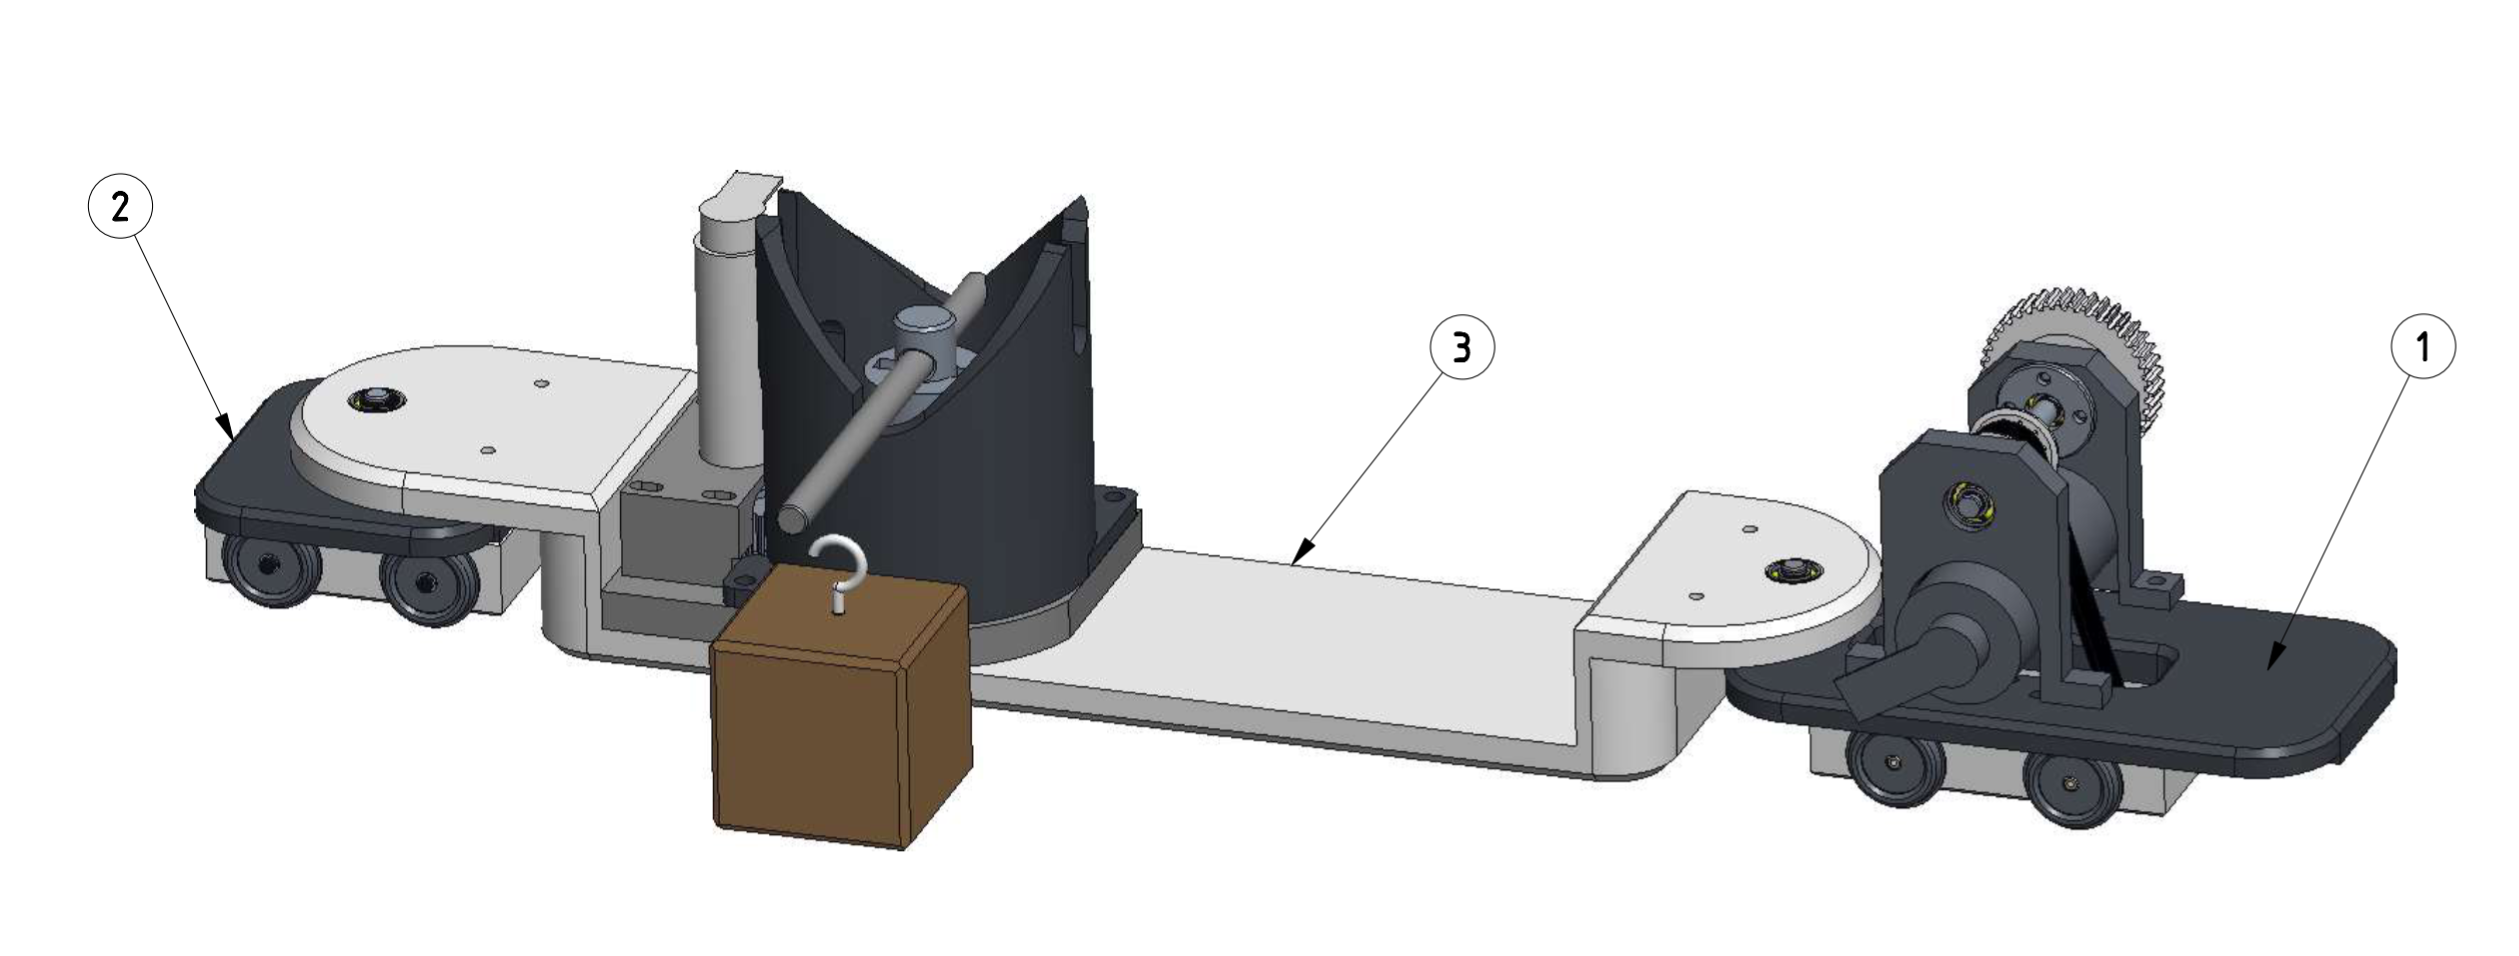
\includegraphics[width=0.82\textwidth]{Lokomotive.png}
        \caption{Baugruppe Lokomotive}
        \label{fig:bg_lokomotive}
    \end{figure}

    \begin{table}[H] \centering
        \begin{tabular}{|l|l|}
        \hline
        \textbf{Position} & \textbf{Bezeichnung}\\
        \hline
        Position 1          & Antriebswagen\\
         \hline
        Position 2          & Führungswagen\\
        \hline
        Position 3          & Ladungsträger\\
        \hline
        Position 4          & Transportgut (Würfel)\\
        \hline
        \end{tabular}

        \caption{Positionsnummern der Lokomotive}
        \label{tab:bg_lokomotive}
    \end{table}

    In der Querschnittsdarstellung in Abbildung \ref{fig:schnitt_lokomotive} sind die Lagerungen zwischen dem Ladungsträger und dem Antriebs- beziehungsweise dem Führungswagen besser sichtbar. Ebenfalls ist ersichtlich, dass der Antriebswagen durch einen Zahnriemen angetrieben wird. Der Aufbau der einzelnen Unterbaugruppen wird in den nächsten Abschnitten genauer vorgestellt.\\

    \begin{figure}[H] %Lokomotive im Schnitt
        \centering
        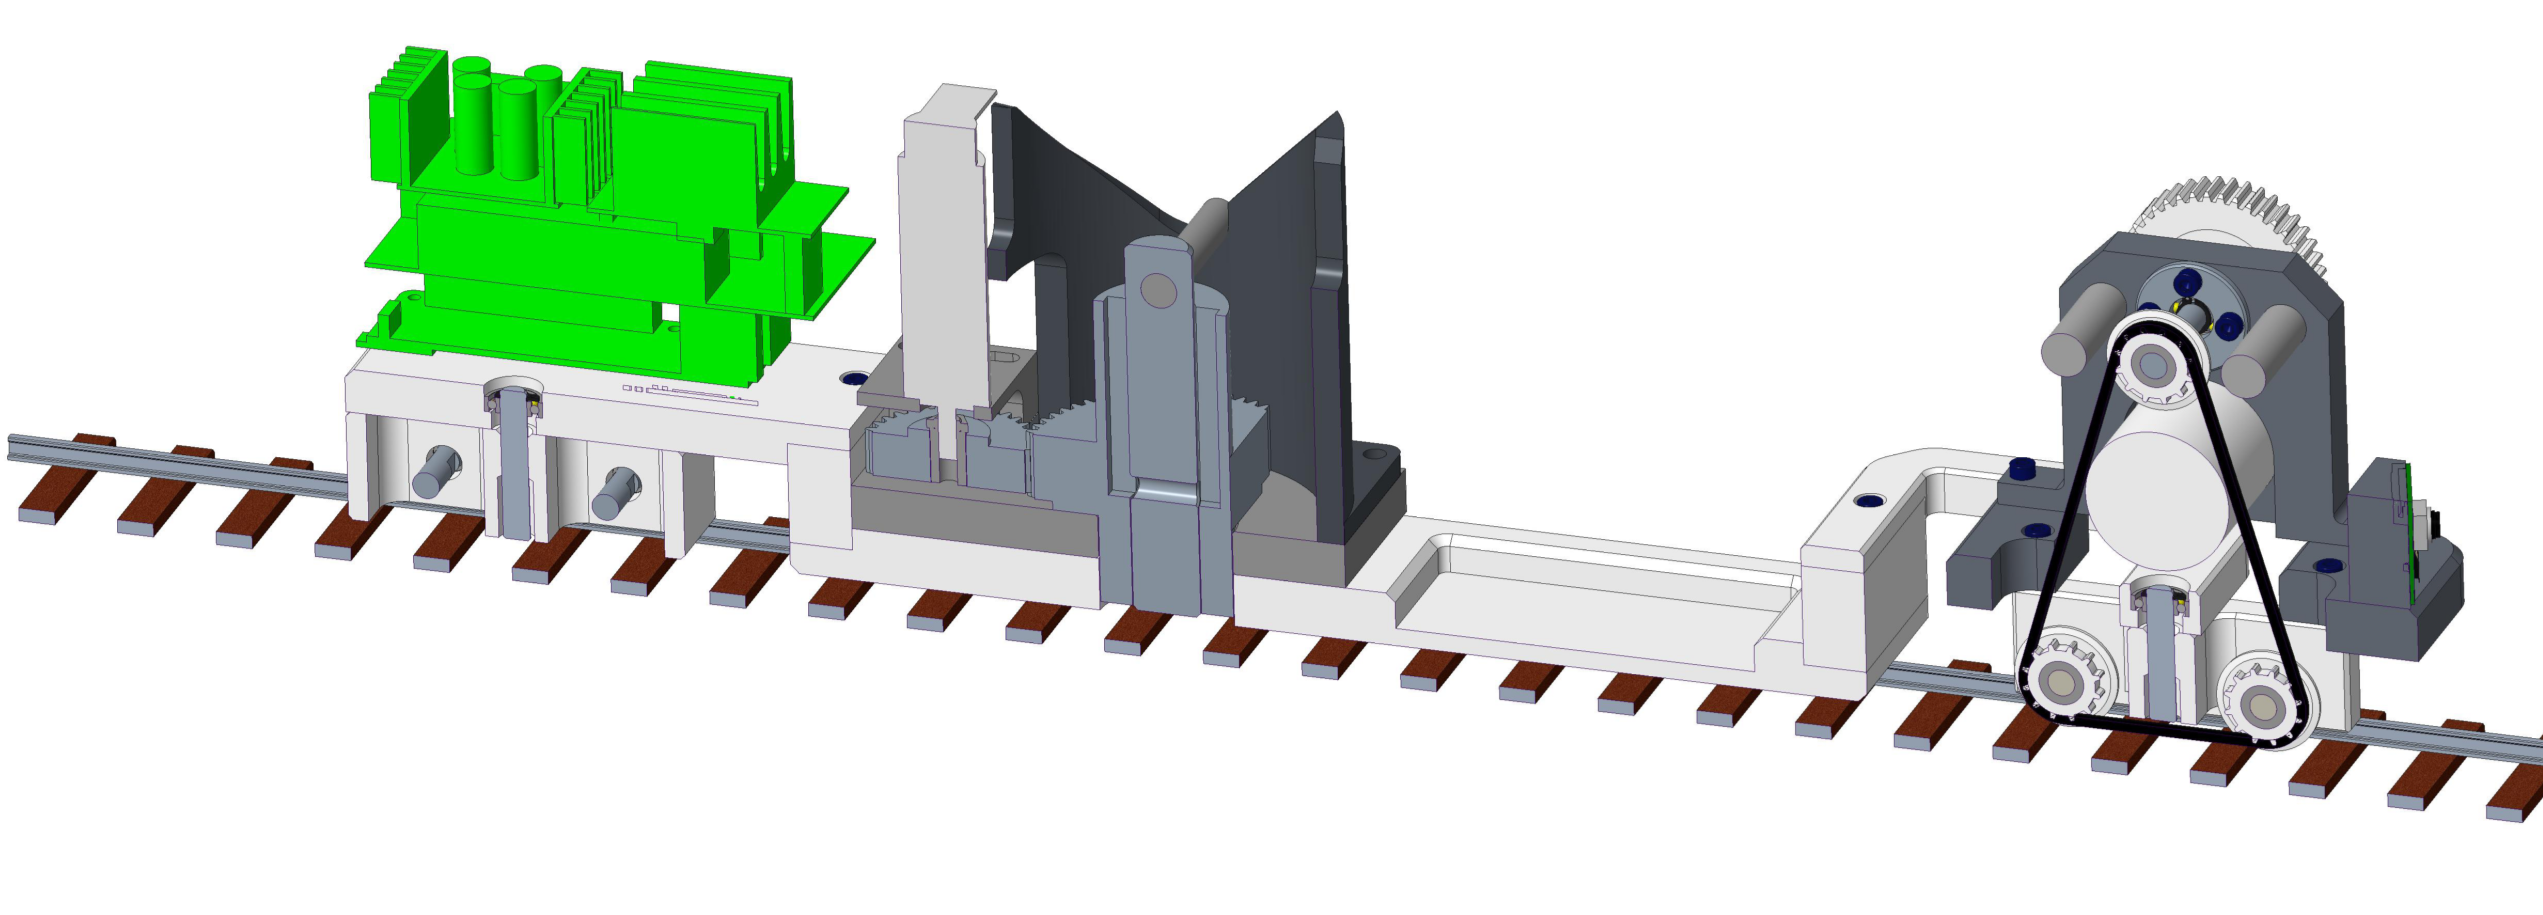
\includegraphics[width=0.82\textwidth]{lokomotive_2.png}
        \caption{Schnittansicht der Lokomotive}
        \label{fig:schnitt_lokomotive}
    \end{figure}
    \newpage

    \subsubsection{Antriebs- und Führungswagen}
    Der Grundaufbau der beiden Wagen ist derselbe, mit dem Unterschied, dass der Antriebswagen durch einen Motor angetrieben wird. Der Grundwagen, beziehungsweise der Führungswagen in Abbildung \ref{fig:expl_fuehrungswagen} (siehe Tabelle \ref{tab:expl_fuehrungswagen}) besteht aus einem Rahmen und einer Platte, welche miteinander verstiftet (Position 2) und verschraubt (Position 3) sind. Im Rahmen werden die beiden Achsen jeweils mit einem Los- (Position 7) und einem Festlager (Position 8) gelagert und mit Sicherungsringen (Position 6) gesichert. Die Achsen sind an beiden Enden mit einem Gewinde versehen, damit die Räder bei Bedarf schnell und einfach gewechselt werden können, ohne dass der ganze Wagen auseinander genommen werden muss. Die Anfräsfläche auf der Welle (Position 5) dient für das bessere Befestigen der Räder mit einen Gabelschlüssel.\\

     \begin{figure}[H] %Führungswagen
        \centering
        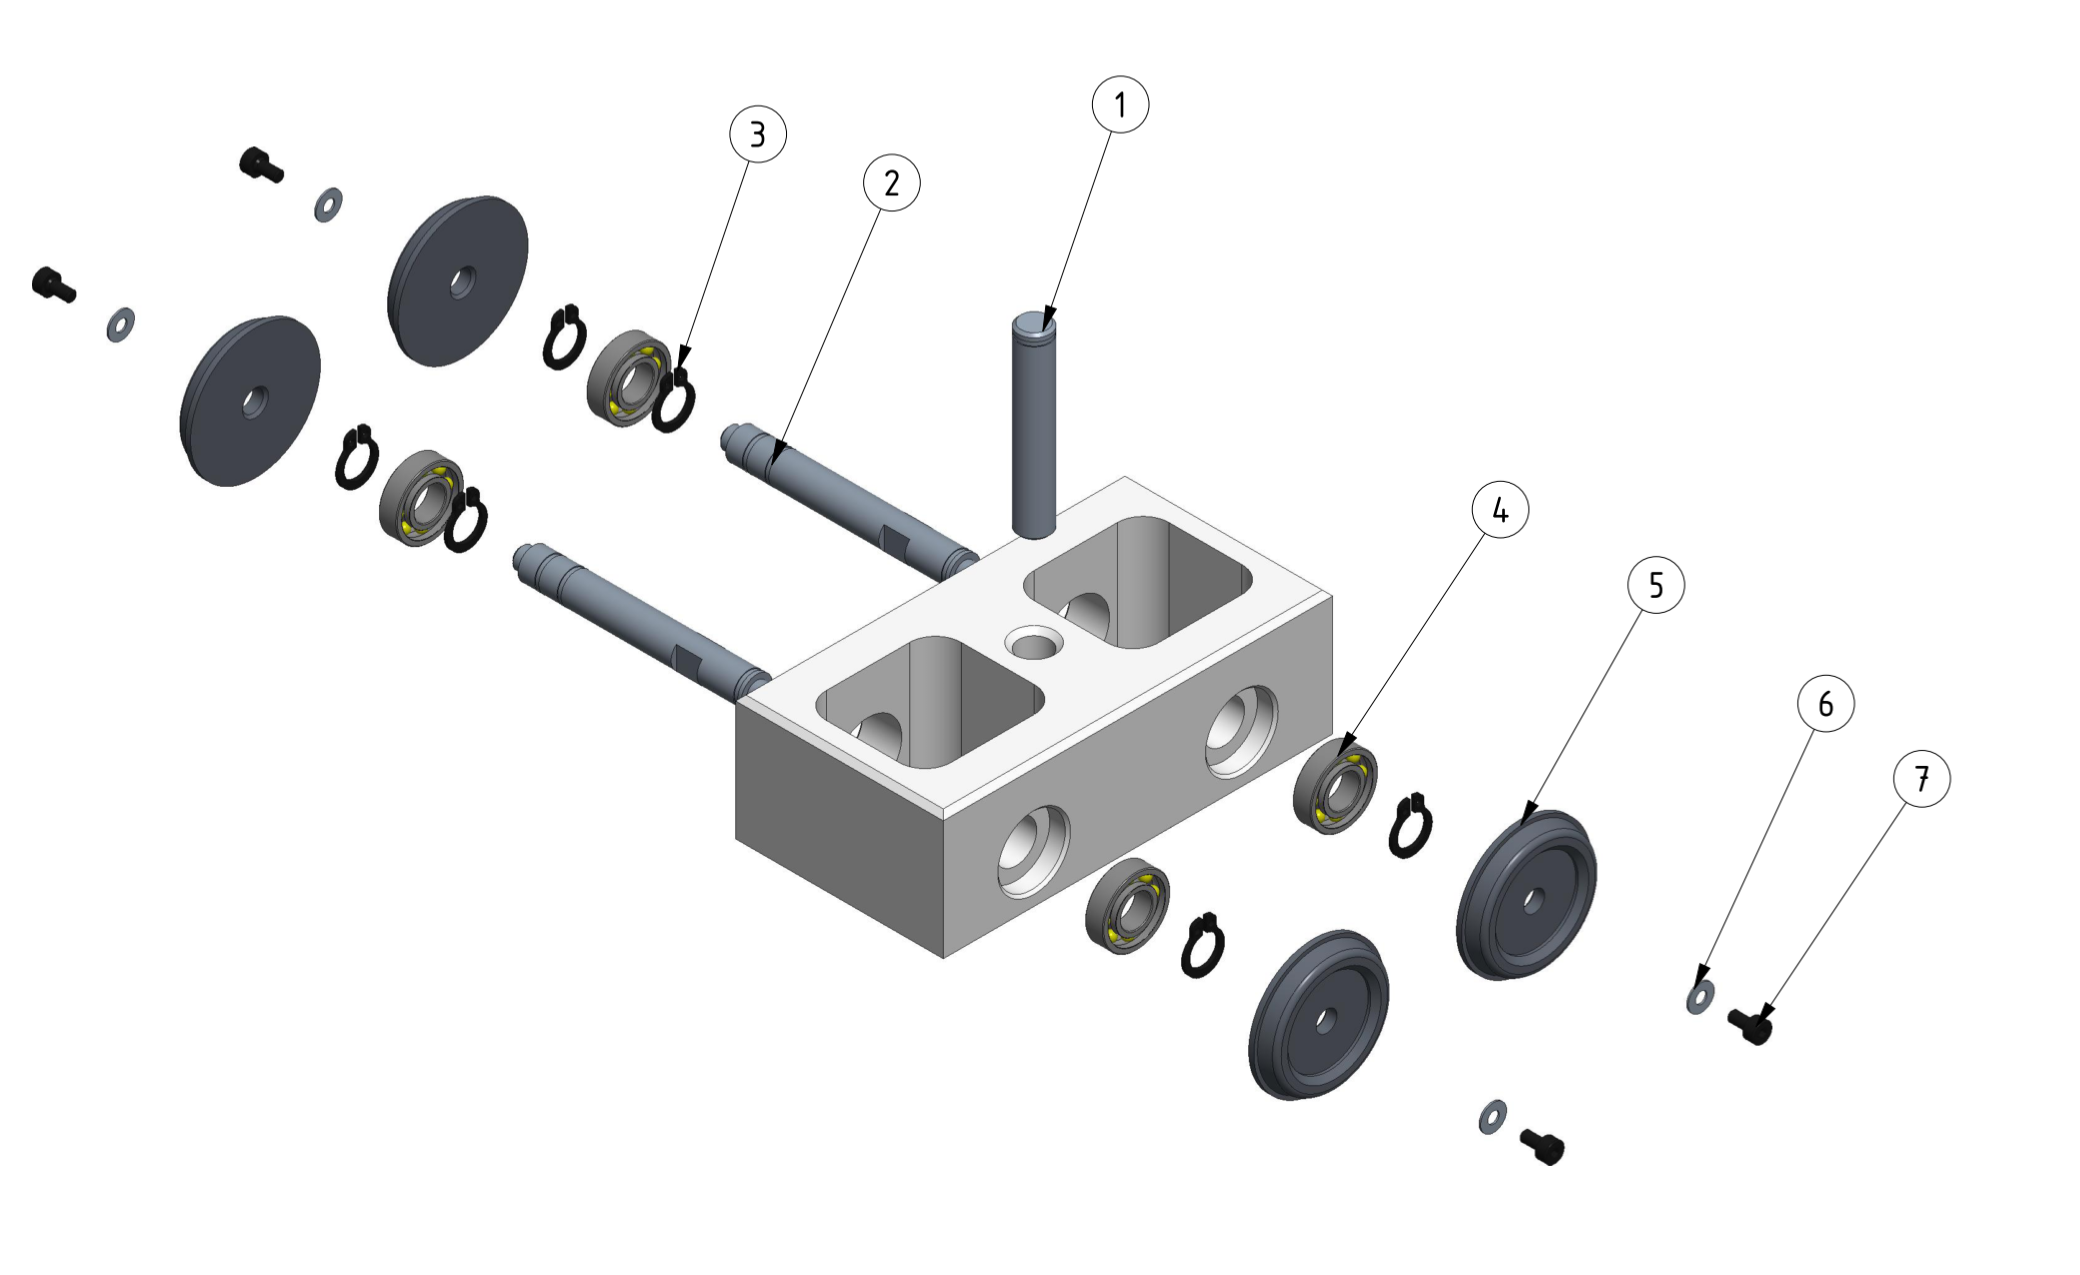
\includegraphics[width=1\textwidth]{Fuehrungswagen.png}
        \caption{Explosionsdarstellung Grundwagens}
        \label{fig:expl_fuehrungswagen}
    \end{figure}

    \begin{table}[H] \centering
        \begin{tabular}{|l|l|}
        \hline
        \textbf{Position} & \textbf{Bezeichnung}\\
        \hline
        Position 1          & Drehachse Wagen-Ladungsträger (eingepresst)\\
         \hline
        Position 2          & Achsen (Gewinde an beiden Seiten, Anfräsfläche für Gabelschlüssel)\\
         \hline
        Position 3          & Sicherungsring für Rillenkugellager\\
        \hline
        Position 4          & Eingepresstes Rillenkugellager (Festlager) bzw. Loslager\\
        \hline
        Position 5          & Rad\\
        \hline
        Position 6          & Unterlagscheibe\\
        \hline
        Position 7          & Zylinderschraube\\
        \hline
        \end{tabular}

        \caption{Positionsnummern des Grundwagens}
        \label{tab:expl_fuehrungswagen}
        \end{table}
    \newpage

    Der Antriebswagen in Abbildung \ref{fig:antriebswagen} (siehe Tabelle \ref{tab:expl_antriebswagen}) ist, wie bereits
    erwähnt, grundsätzlich gleich aufgebaut wie der Führungswagen. Jedoch ist der Rahmen aufgrund des Riemenantriebs
    H-Förmig aufgebaut. Das heisst, die beiden Nuten des Wagenrahmens sind nach Aussen hin offen. Das Ziel dieser
    Konstruktion ist es den Riemen, falls nötig, schnell wechselbar zu montieren. Durch die H-Form können die Achsen und
    die Räder für die Riemenmontage am Rahmen montiert bleiben. Die Platte, welche am Rahmen angebracht ist,
    ist für die Kameras grösserer Dimensioniert. Die Kamera für die Gleiserkennung wird
    einstellbar befestigt, damit bei der Testphase des Prototyps Optimierungen des Winkels vorgenommen werden können.
    Die Kamera für die Signalerkennung wird fix montiert.
    Der Stromfluss von der Schiene auf die Lokomotive erfolgt über vier Schleifkontakte, welche als Einkaufsteile von
    Lieferanten bezogen werden. Davon sind pro Wagen zwei jeweils zwischen den Rädern angebracht.\\

    \begin{figure}[H] %Antriebswagen
        \centering
        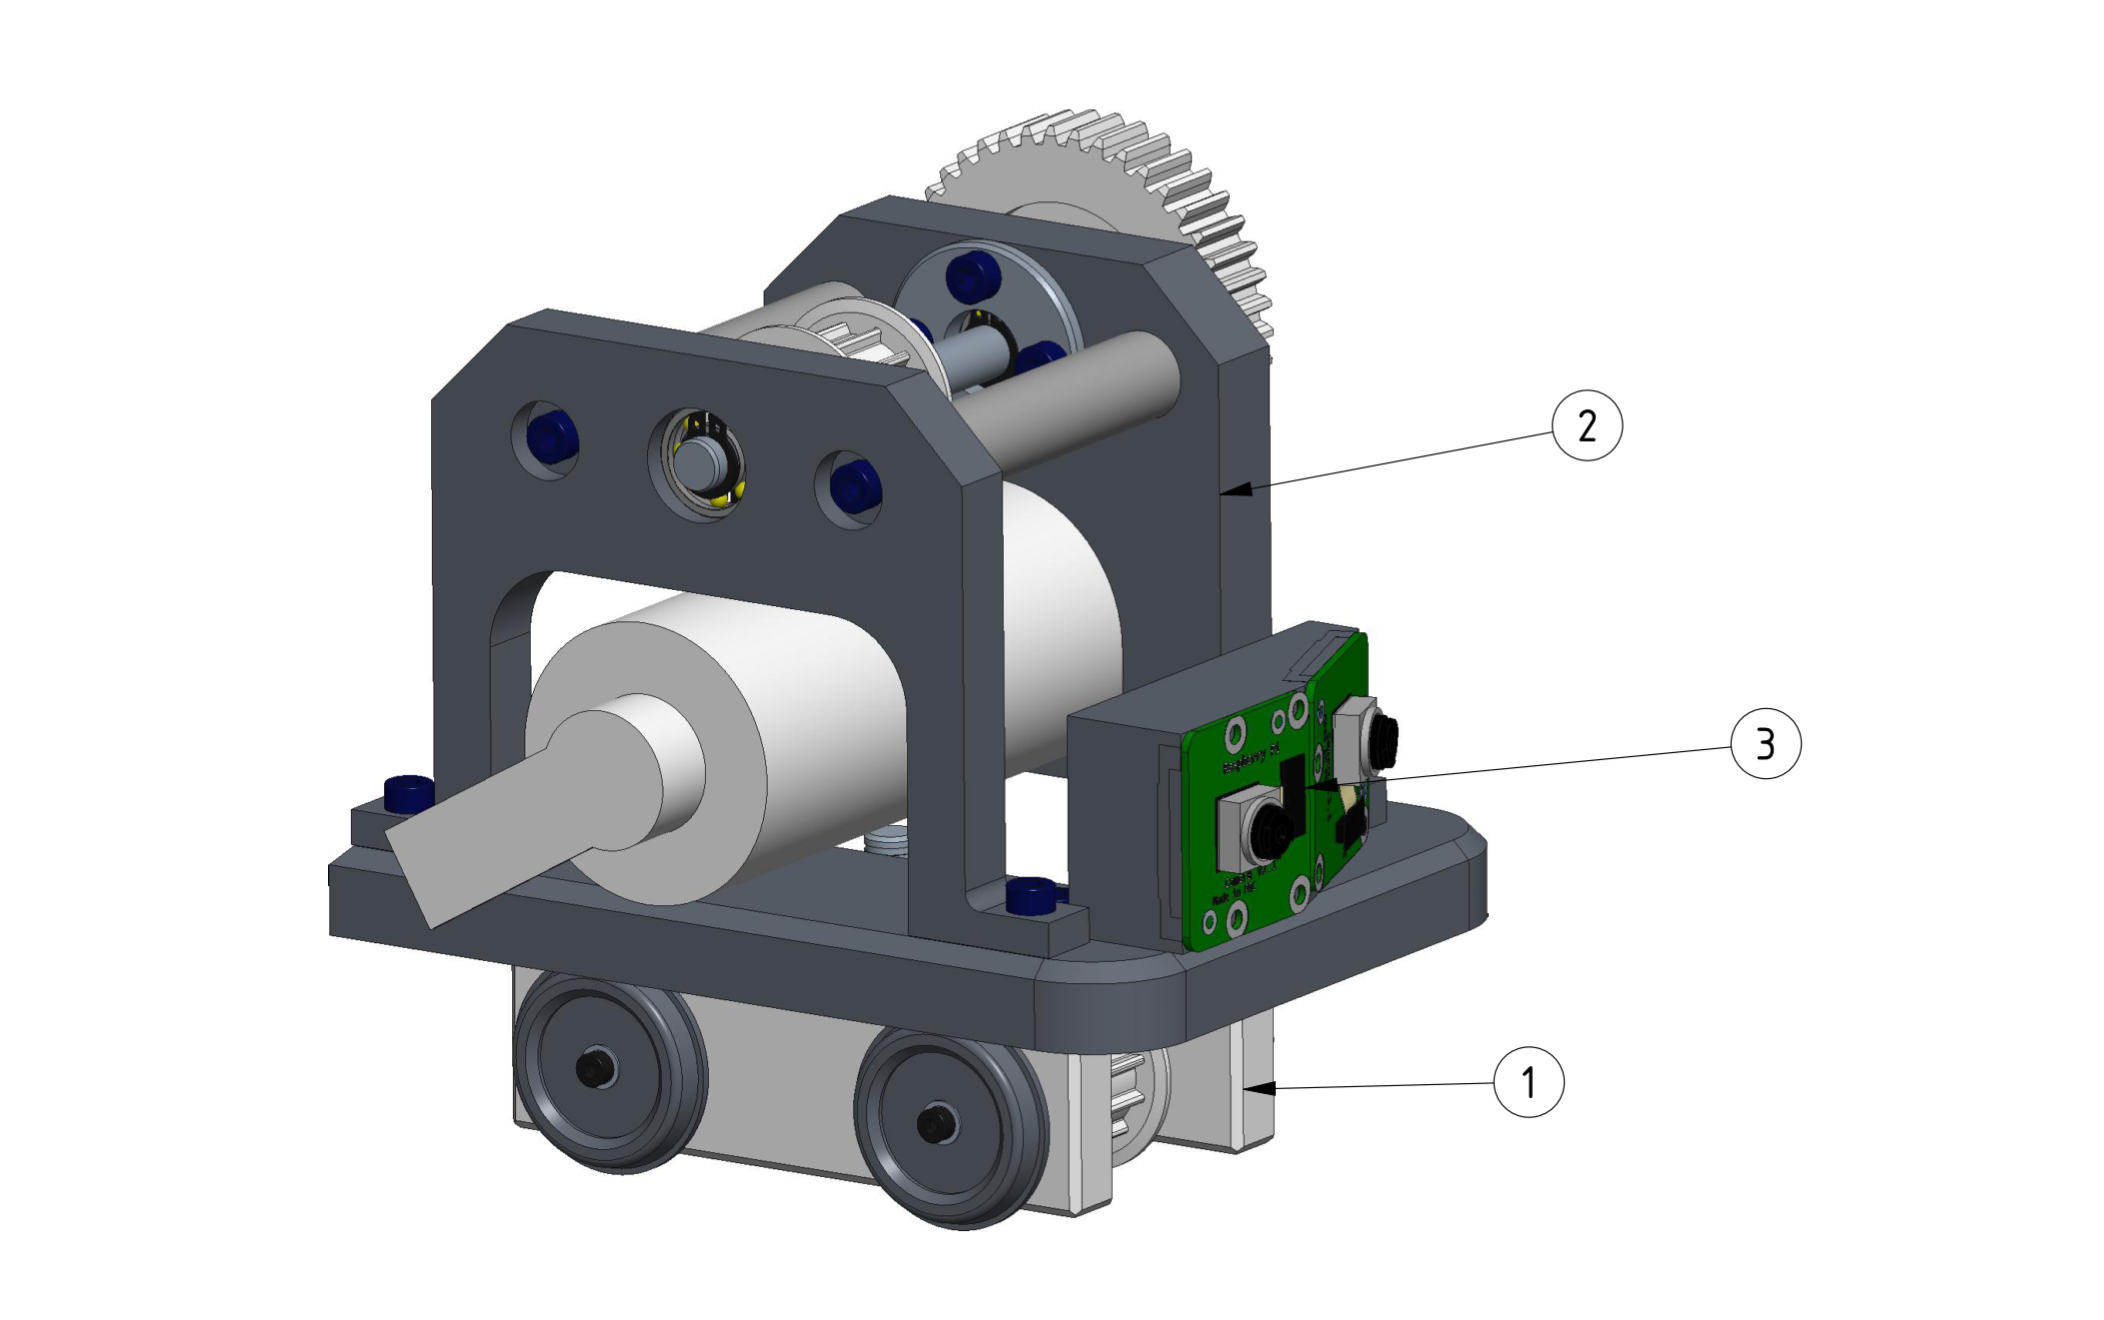
\includegraphics[width=0.7\textwidth]{antriebswagen.png}
        \caption{Baugruppe Antriebswagen}
        \label{fig:antriebswagen}
    \end{figure}

    \begin{table}[H] \centering
        \begin{tabular}{|l|l|}
        \hline
        \textbf{Position} & \textbf{Bezeichnung}\\
        \hline
        Position 1          & Wagen\\
         \hline
        Position 2          & Antriebseinheit\\
        \hline
        Position 3          & Kameras\\
        \hline
        Position 4          & Zahnriemen\\
        \hline
    \end{tabular}

    \caption{Positionsnummern des Antriebswagens}
    \label{tab:expl_antriebswagen}
    \end{table}

    \pagebreak

    Die Antriebseinheit in Abbildung \ref{fig:antriebseinheit} (siehe Tabelle \ref{tab:pos_antriebseinheit}) besteht aus einem Grundgestell, an welchem die Lagerung der Antriebswelle und der Motor angebracht sind. Das Drehmoment vom Motor wird über ein geradverzahntes Zahnrad mit einem Übersetzungsverhältnis von 1:2 auf eine Achse übertragen. Von dieser wird es über einen Riemen auf die beiden Radachsen und somit auf die Räder weitergeleitet. Durch die Berechnung der maximalen Geschwindigkeit wird entsprechend der Motor ausgelegt. Dies wird im nächsten Abschnitt genauer beschrieben.\\

    \begin{figure}[H] %Antriebseinheit
        \centering
        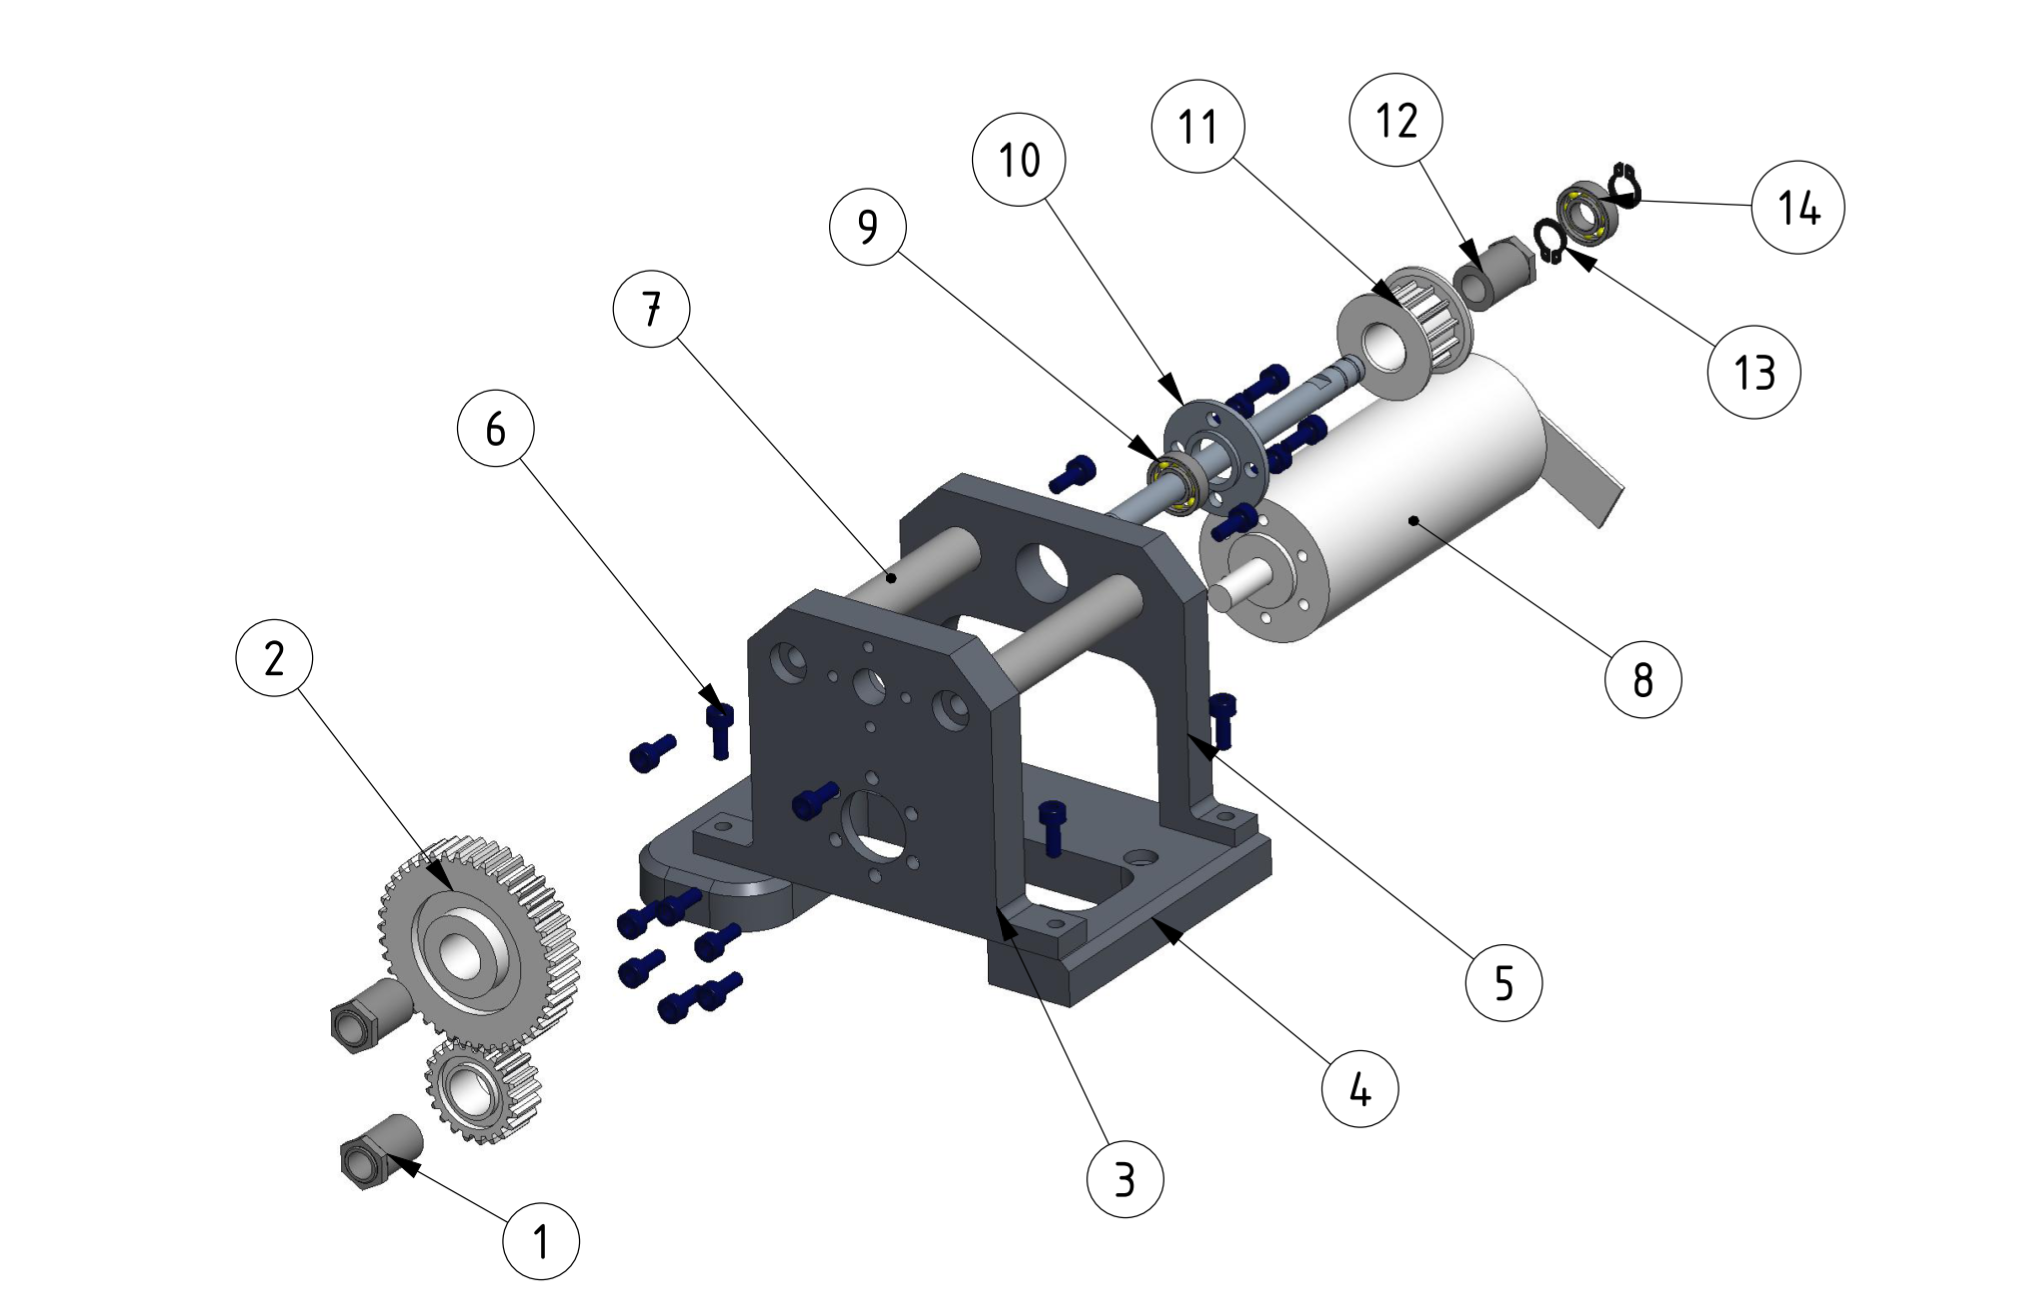
\includegraphics[width=1\textwidth]{antriebseinheit.png}
        \caption{Explosionsdarstellung Antriebseinheit}
        \label{fig:antriebseinheit}
    \end{figure}

    \begin{table}[H] \centering
        \begin{tabular}{|l|l|}
        \hline
        \textbf{Position} & \textbf{Bezeichnung}\\
        \hline
        Position 1          & Spannsatz\\
         \hline
        Position 2          & Zahnräder (Übersetzung 1:2)\\
        \hline
        Position 3          & Motorhalterung\\
        \hline
        Position 4          & Grundplatte\\
        \hline
        Position 5          & Achsenlagerplatte\\
        \hline
        Position 6          & Zylinderschraube\\
        \hline
        Position 7          & Distanzhülsen\\
        \hline
        Position 8          & Motor\\
        \hline
        Position 9          & Rillenkugellager (Loslager)\\
        \hline
        Position 10         & Lagersicherungsplatte\\
        \hline
        Position 11         & Zahnriemenrad\\
        \hline
        Position 12         & Spannsatz\\
        \hline
        Position 13         & Sicherungsring\\
        \hline
        Position 14         & Rillenkugellager (Festlager)\\
        \hline
        \end{tabular}

        \caption{Positionen Antriebseinheit}
        \label{tab:pos_antriebseinheit}
        \end{table}

    \pagebreak

    \textbf{Beschleunigungsberechnung}\\
    Wie schnell die Lokomotive beschleunigen kann, hängt von der Reibung zwischen Rad und Schiene und der Masse des Zuges ab. Die Grunddefinition der Beschleunigung ist der Quotient von Kraft und Masse. Die Reibung ist durch den Reibkoeffizienten bestimmt, welcher sich von Materialpaarung zu Materialpaarung unterscheidet (siehe Tabelle \ref{tab:reibungskoeffizient}). Zusätzlich ist der Reibkoeffizient von der Oberflächenbeschaffenheit, der Rauigkeit, abhängig. Je grösser die Rauigkeit, desto mehr Reibung entsteht und desto schneller kann beschleunigt werden.\\

    \begin{table}[H] \centering
        \begin{tabular}{|l|l|l|}
        \hline
        \textbf{Material Schiene} & \textbf{Material Rad} & \textbf{Reibungskoeffizient}\\
        \hline
        Stahl                                & Stahl        & 0.12\\
        \hline
        Stahl                                & Holz         & 0.3\\
        \hline
        Stahl                                & Kunststoff   & 0.08\\
        \hline
        Stahl                                & Gummi        & 0.3\\
        \hline
        \end{tabular}

        \caption{Reibungskoeffizienten von Materialpaarungen (durch Versuche ermittelt)}
        \label{tab:reibungskoeffizient}
        \end{table}

    Um die maximale Beschleunigung zu berechnen, wird das Gesamtgewicht der Lokomotive auf die vier Räder aufgeteilt. In der Tabelle \ref{tab:groessen_beschleunigung} sind die gegeben Grössen für die nachfolgenden Berechnungen aufgelistet.\\

    \begin{table}[H] \centering
        \begin{tabular}{|l|l|}
        \hline
        \textbf{Grösse} & \textbf{Wert}\\
        \hline
        Durchmesser Rad [D]          & 22 Milimeter\\
         \hline
        Reibungskoeffizient [k]      & 0.3\\
        \hline
        \end{tabular}

        \caption{Grössen für die Beschleunigungsberechnung}
        \label{tab:groessen_beschleunigung}
        \end{table}

    $$F_{Rad}=\frac{F_{G}}{8}=\frac{m \cdot g=3kg \cdot 9.81m/s^2}{8}=0.375N$$

    $$F_{Reibung}=F_{Rad} \cdot k=0.375N \cdot 0.3=0.1125N$$

    $$M_{Rad}=F_{Rad} \cdot 0.5 \cdot D_{Rad}= 0.1125N \cdot 0.5 \cdot 22mm = 1.24mNm$$

    $$a_{max}=\frac{F_{Reibung}}{\frac{F_{Rad}}{g}}=\frac{0.1125N}{\frac{0.375N}{9.81m/s^2}}=2.94m/s^2$$
    \\

    \label{GeschwindigkeitsberechnungFahrwerk}
    \textbf{Geschwindigkeitsberechnung}\\
    Die Fahrgeschwindigkeit der Lokomotive wird durch zwei Faktoren bestimmt. Einerseits muss die maximale Geschwindigkeit der Anforderungsliste eingehalten werden, und andererseits wird die Geschwindigkeit in der Kurvenfahrt durch den Schwerpunkt des Fahrzeuges eingeschränkt. Nachdem die Lokomotive auf die Fahrtgeschwindigkeit beschleunigt wurde, ist die Rollreibung das einzige, was der Motor mit seiner Leistung kompensieren muss. In der Anforderungsliste wurde eine minimale Geschwindigkeit von 0.5 Meter pro Sekunde festgelegt. Der begrenzende Faktor der Geschwindigkeit in der Kurve ist der Schwerpunkt der Lokomotive. Je tiefer dieser ist, umso schneller kann die Kurve abgefahren werden. Über die Zentripedalkraft und die Gewichtskraft der Lokomotive wird die Momentengleichung aufgestellt und Anhand der gegebenen Werte in Tabelle \ref{tab:geschwindigkeitsberechnung} wird die maximal erreichbare Geschwindigkeit in der Kurve, ohne aus den Gleisen zu kippen, berechnet. Sie sind durch getroffene Annahmen entstanden, da noch nicht alle Koponenten und die dazugehörige Massen festgelgt sind.\\
    Das Kippmoment wird durch den Aufbau der Lokomotive minimiert, da der Schwerpunkt durch den Ladungsträger mehr in das Zentrum des Kreismittelpunktes rückt. Dies wird in den nachfolgenden Berechnungen nicht berücksichtigt.\\

    \begin{figure}[H] %Schwerpunkt
        \centering
        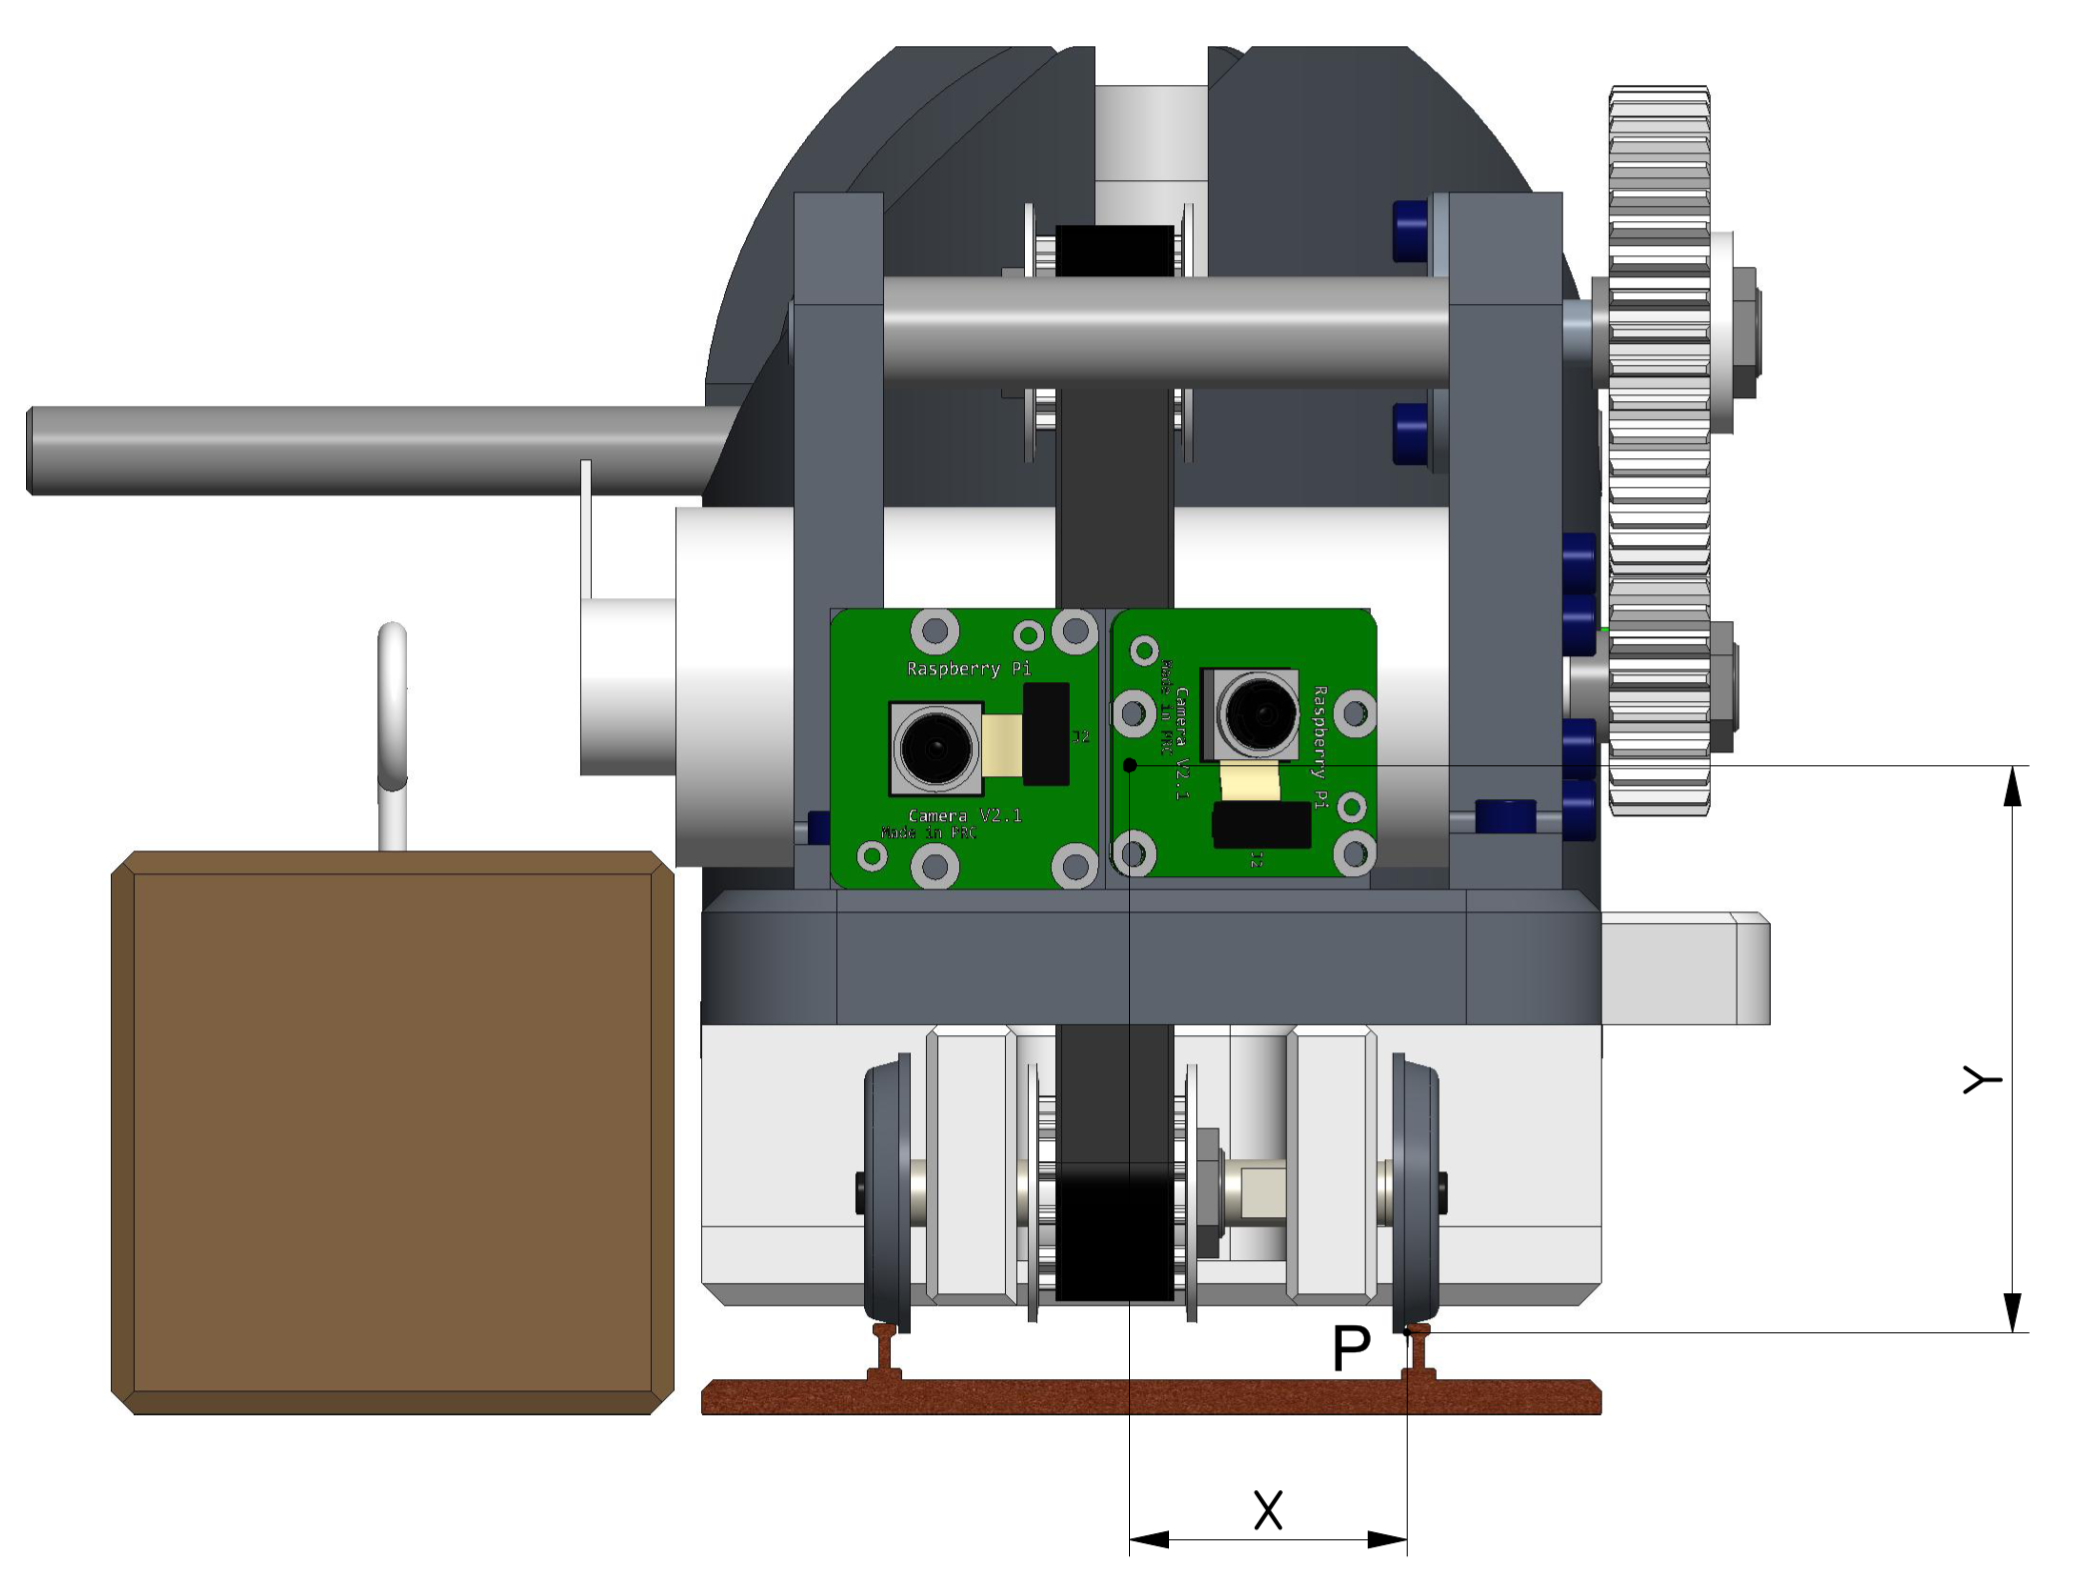
\includegraphics[width=0.65\textwidth]{schwerpunkt.png}
        \caption{Schwerpunkt der Lokomotive (Symbolisch)}
        \label{fig:schwerpunkt}
    \end{figure}

    \begin{table}[H] \centering
        \begin{tabular}{|l|l|}
        \hline
        \textbf{Grösse} & \textbf{Wert}\\
        \hline
        Minimaler Radius  [r]                               & 0.8 Meter\\
         \hline
        Masse [m]                                           & 3 Kilogramm\\
        \hline
        Schwerpunkt in x-Achse (maximaler Wert) [x]         & 0.0225 Meter\\
        \hline
        Schwerpunkt in y-Achse (maximaler Wert) [y]         & 0.05 Meter\\
        \hline
        \end{tabular}

        \caption{Grössen für die Geschwindigkeitsberechnung}
        \label{tab:geschwindigkeitsberechnung}
        \end{table}

    Die Gewichts- und Zentripedalkraft, welche das Gleichungssystem für die Geschwindigkeitsberechnung bilden, sind wie folgt definiert:

    $$F_{G}=m \cdot g=3kg \cdot 9.81m/s^2=29.4N$$

    $$F_{max, z}=\frac{F_{G} \cdot x}{y}=\frac{29.4N \cdot 0.0225m}{0.05m}=13.24N$$
    \newpage

    Da das Drehmoment eine vektorielle Grösse ist, müssen die beiden entstehenden Momente am Drehpunkt ''P'' am Gleis zusammen Null ergeben. Oder anders gesagt, müssen die beiden Momente gleich gross sein, damit das System ''statisch'' bestimmt ist. Die Berechnungen sind auf den kleinsten Kurvenradius ausgelegt, da dort die grösste Zentripedalkraft entsteht. Somit ergibt sich eine maximale Geschwindigkeit von 1.53 Meter pro Sekunde.

    $$F_{max, z}=\frac{m \cdot v_{max}^2}{r}$$

    $$v_{max}=\sqrt\frac{F_{max, z}\cdot r}{m}=\sqrt\frac{13.24N \cdot 0.8m}{3kg}=1.53m/s$$

    \subsubsection{Ladungsträger}
    Der Ladungsträger ist das Verbindungselement von Antriebswagen und Führungswagen. Er wird an beiden Enden drehbar mit je einem Radiallager gelagert. Die Flächen der Platten reiben auf den beiden Wagen. Durch eine optimale Materialpaarung wird diese Reibkraft jedoch vernachlässigbar klein. Der Träger besteht aus den drei Teilen mit Position 1,3 und 7 (siehe Abbidlung \ref{fig:expl_ladungstraeger}), welche durch Zylinderschrauben (Position 5) und einer Zwischenplatte (Position 2) zusammengebaut wird. Der Hauptgrund ist die einfachere, materialsparende sowie kostengünstigere Herstellung.\\

    \begin{figure}[H] %Ladungsträger
        \centering
        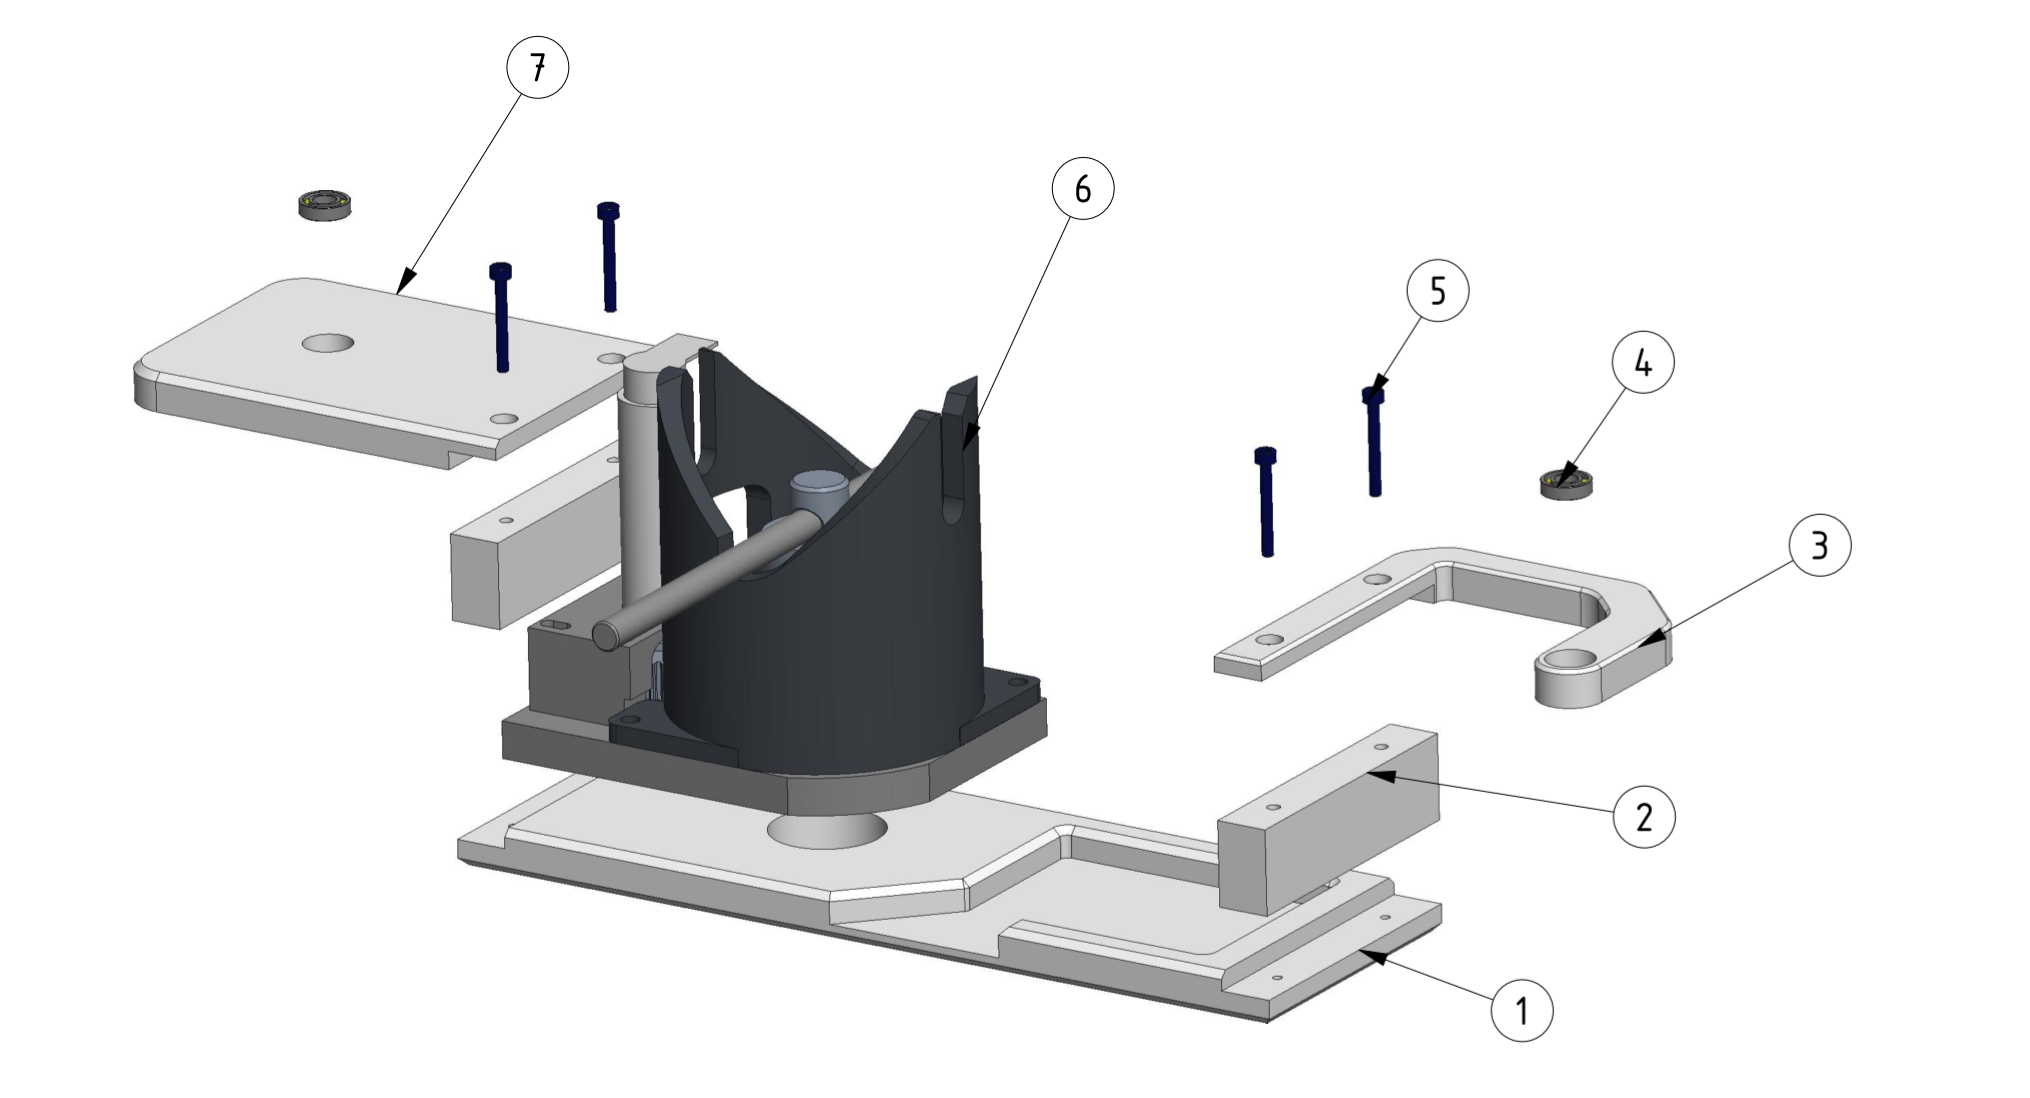
\includegraphics[width=0.75\textwidth]{ladungstraeger.png}
        \caption{Explosionsdarstellung Ladungsträger}
        \label{fig:expl_ladungstraeger}
    \end{figure}
    \begin{table}[H] \centering
        \begin{tabular}{|l|l|}
        \hline
        \textbf{Position} & \textbf{Bezeichnung}\\
        \hline
        Position 1          & Grundplatte\\
         \hline
        Position 2          & Zwischenplatte\\
        \hline
        Position 3          & Bügelgelenk\\
        \hline
        Position 4          & Rillenkugellager\\
        \hline
        Position 5          & Zylinderschrauben\\
        \hline
        Position 6          & Würfelkran\\
        \hline
        Position 7          & Plattengelenk\\
        \hline
        \end{tabular}

        \caption{Positionen des Ladungsträgers}
        \label{tab:pos_ladungstraeger}
        \end{table}

\end{document}